% Replace only the old figure carrying fig:bandwidth-appendix-diagnostic.
% Requires graphicx. Keep the existing appendix equations and proofs.

\begin{figure}[tbp]
  \centering
  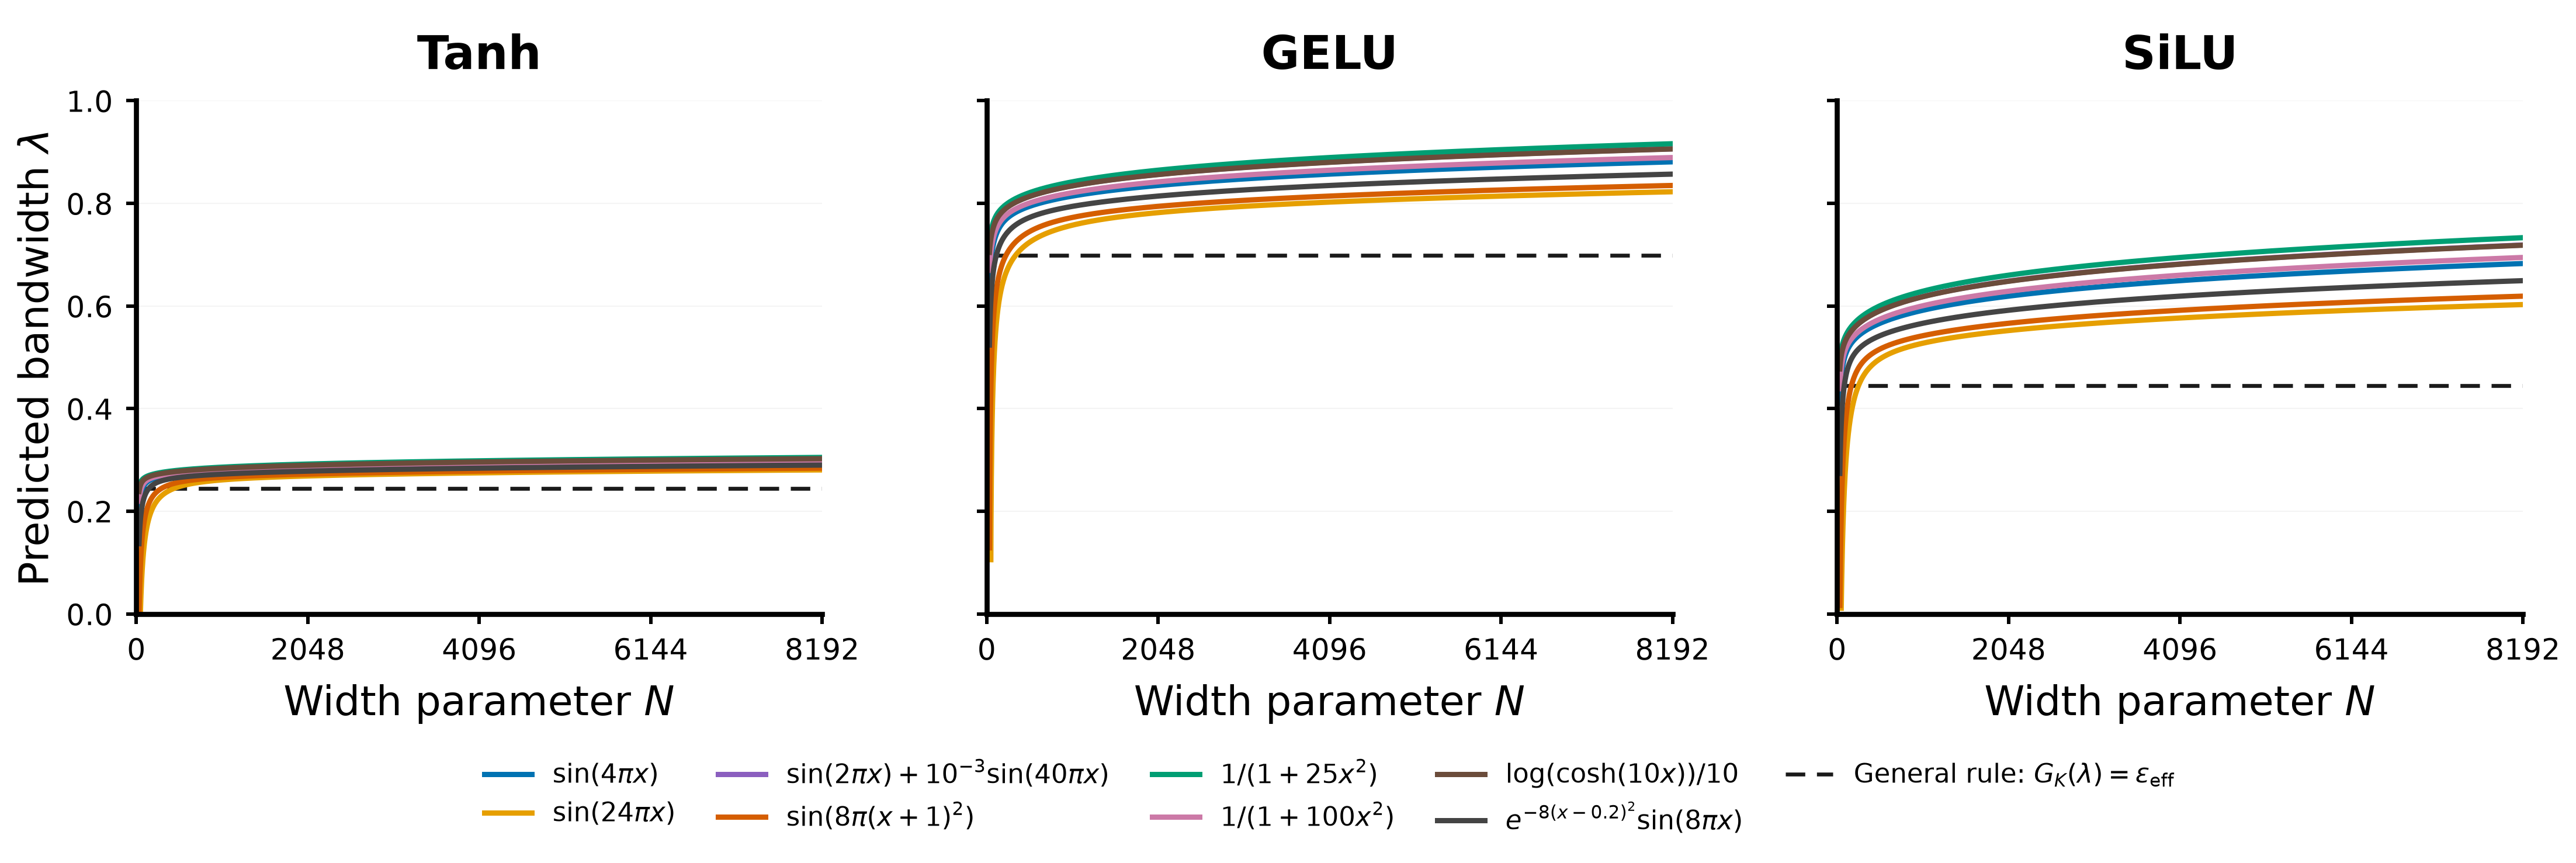
\includegraphics[width=\linewidth]{figures/bandwidth_width_rules.png}
  \caption{Bandwidth selection versus width parameter $N$ for tanh,
  exact GELU, and SiLU. Colored curves give the refined selections for
  the eight targets in the legend, using $\varepsilon_{\rm eff}=2^{-52}$.
  Dashed lines give the activation-specific general-rule selections
  (approximately $0.25$ for tanh). These are scalar rule calculations,
  not fitted-network errors; the refined selections retain their
  frequency-dependent drift.}
  \label{fig:bw-width-rules}
\end{figure}

\begin{figure}[tbp]
  \centering
  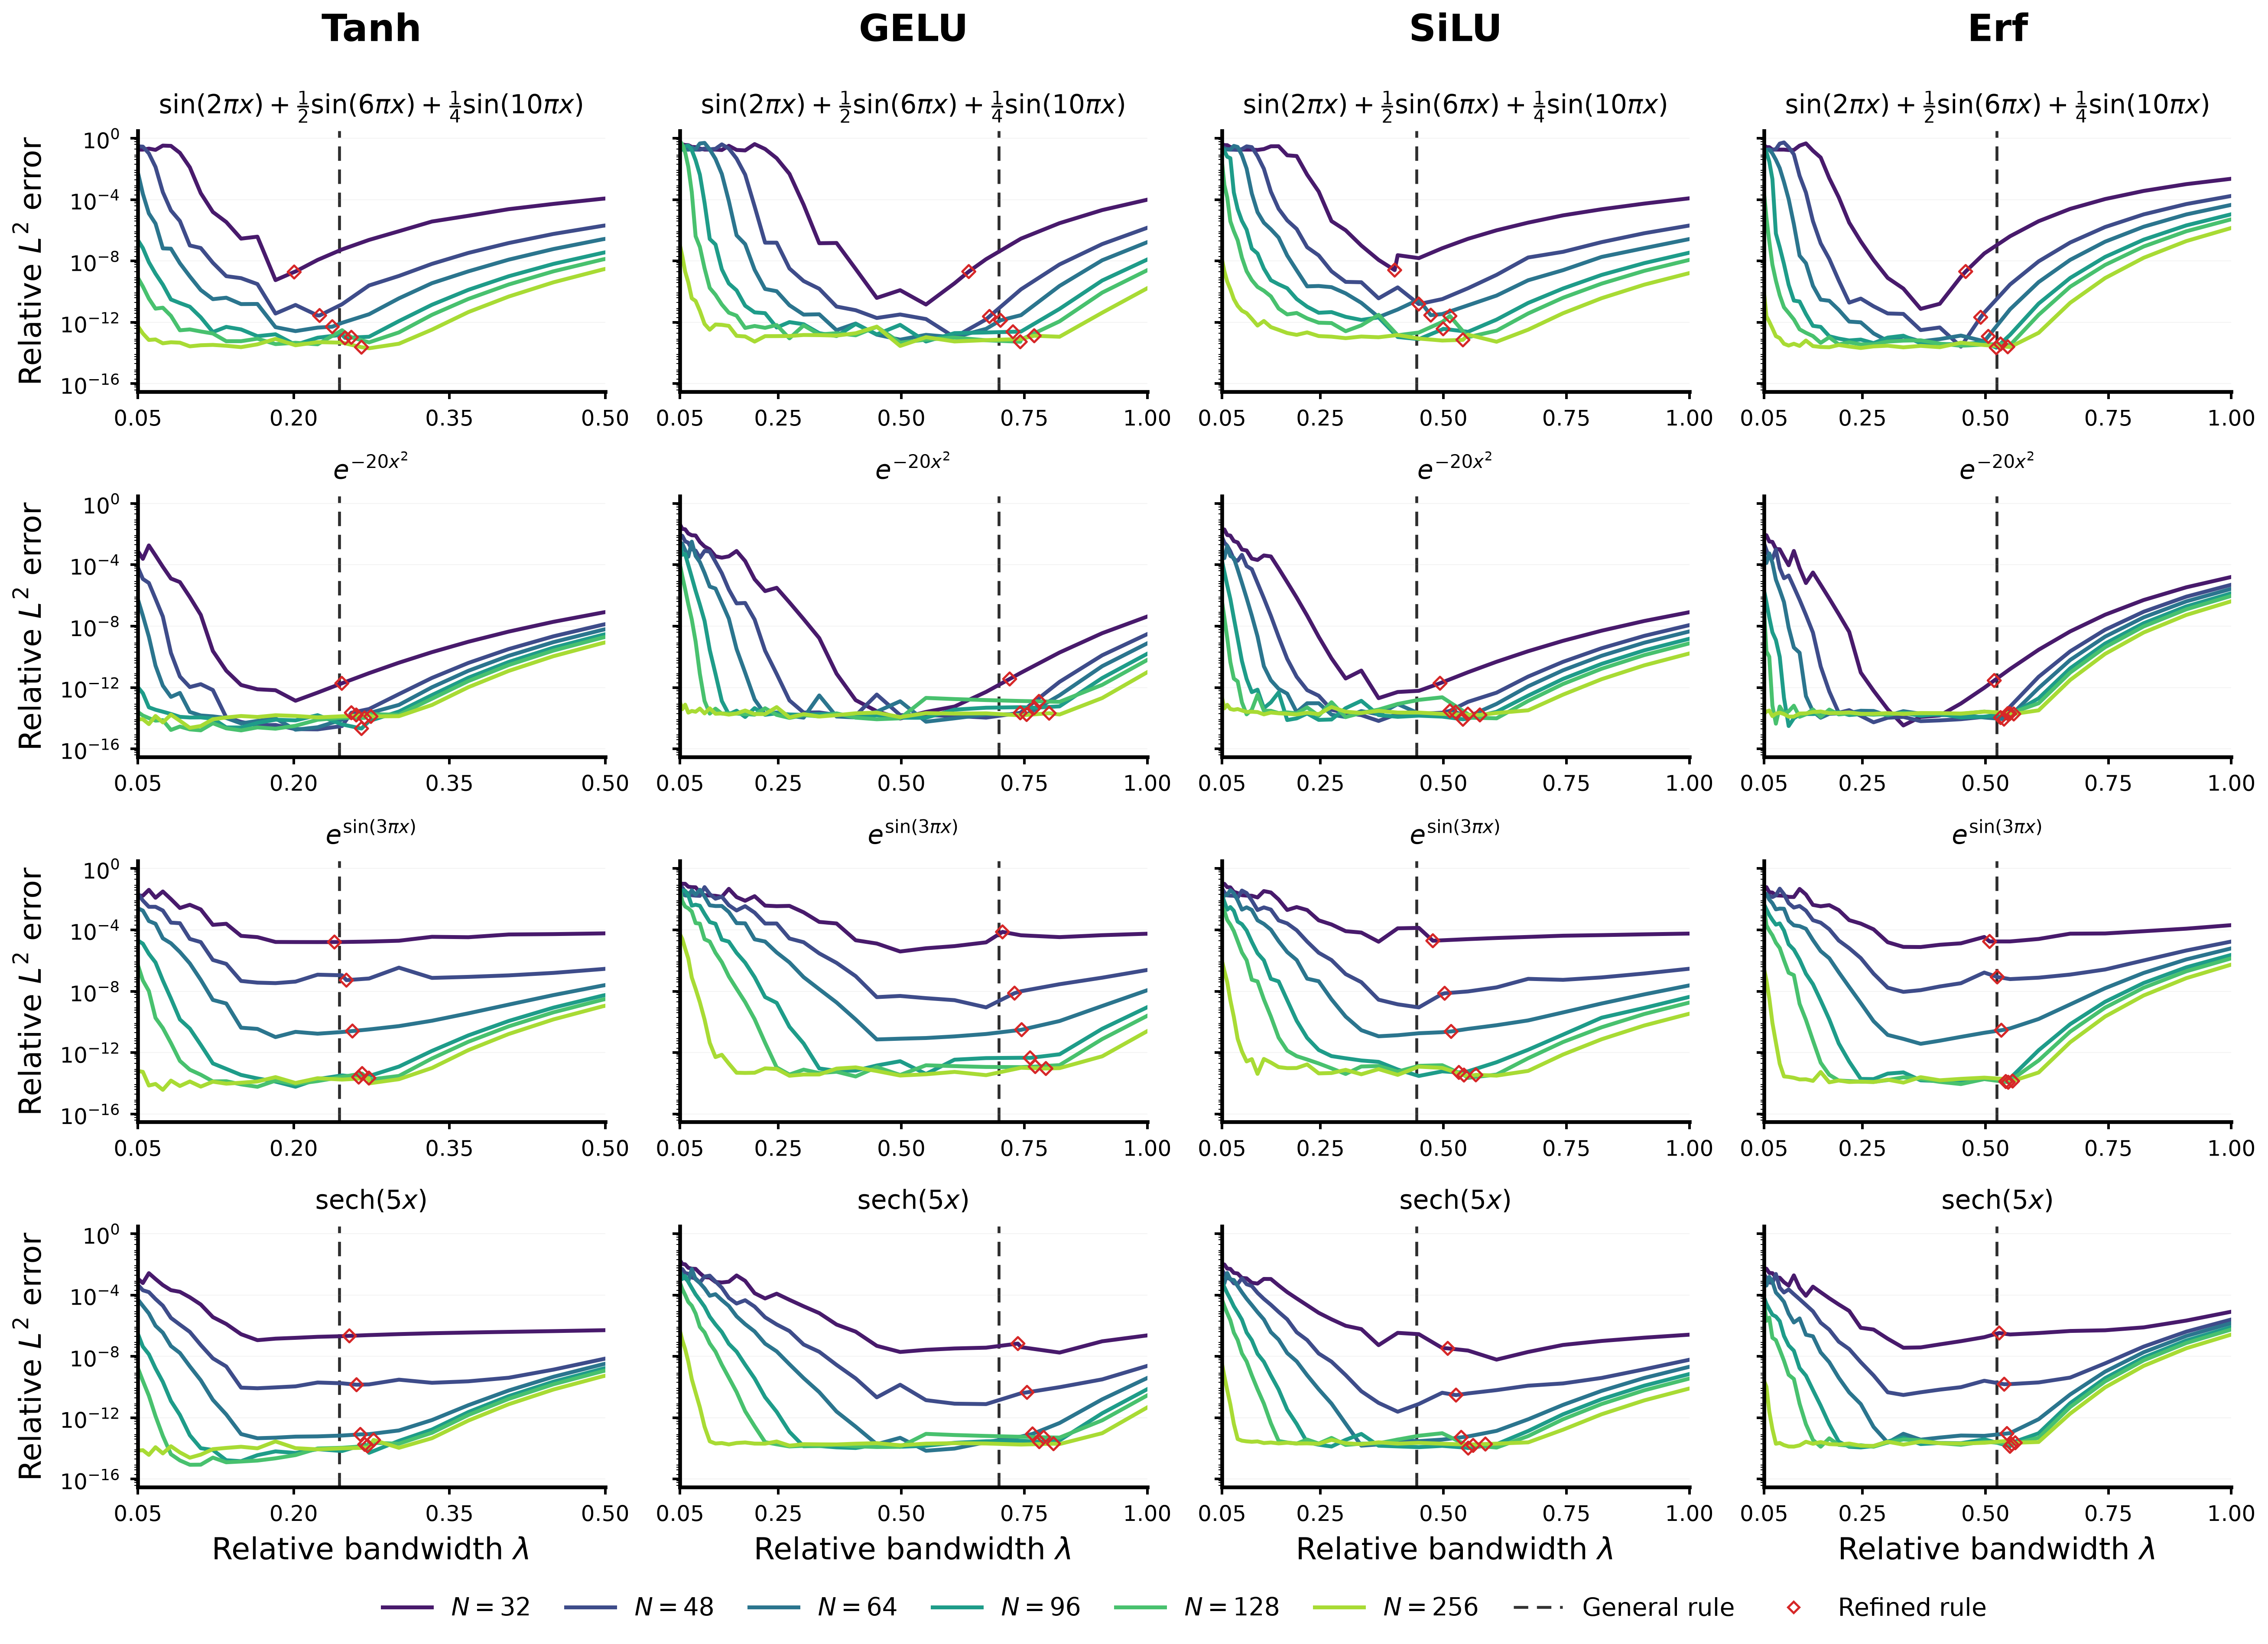
\includegraphics[width=\linewidth]{figures/bandwidth_error_rules.png}
  \caption{Measured relative $L^2$ error versus bandwidth for four
  targets (rows) and four activations (columns). Colors indicate
  $N=32,48,64,96,128,256$, with 32 halo nodes per side and total width
  $W=N+65$. Vertical dashed lines mark the general rule; red diamonds
  mark the refined selections and their directly measured errors.
  Readouts use FP64 SVD least squares on 2003 uniform points, with
  relative singular-value cutoff $2^{-52}$; errors use 4001 uniform
  evaluation points. Tanh is shown over $0.05\le\lambda\le0.5$;
  the other activations extend to $1$. Refined selections use the
  representative-frequency heuristic and need not minimize measured error.}
  \label{fig:bw-error-rules}
\end{figure}
